\section{Interaction Model}
\label{sec:solution:interaction}

An analytical surface composed of independent visualizations is less
useful than the same surface with coordinated interactions across
visualizations. The user expects three behaviors: a click on an
analytical entity opens a multi-chart summary in one place; an unusual
point carries an explanatory hint; the user's filter and selection
choices persist as they navigate through the theme. The proposed
system meets these expectations by composing three interaction
patterns into a single layer. The first is the click-to-entity-detail
panel, which realizes the Connect category of the Yi (2007)
seven-category taxonomy~\cite{yi2007interaction} without simultaneous
cross-chart propagation. The second is a set of visual-storytelling
invariants applied per chart. The third is a theme-scoped state model
that carries the user's filter and selection choices across the
chart-by-chart navigation within a theme.

\subsection{Coordination}
\label{sec:solution:interaction:mcv}

The Multiple Coordinated Views (MCV) pattern surveyed in
Chapter~\ref{chapter:foundations}~\cite{liu2022} composes the Yi (2007)
Connect category as simultaneous propagation across sibling charts: a
selection in one view updates every other view rendered on the same
screen at the same time. The proposed system retains MCV as
intellectual lineage but does not implement the simultaneous form. The
user interface renders one chart per canvas at any time
(Section~\ref{sec:solution:overview}), so propagation across
simultaneously rendered siblings is not visible to the reader. A
coordination model that requires invisible state changes to several
charts the user cannot currently see would expend implementation
complexity for no perceptible analytical gain. The literature
recognizes that the Connect intent admits several realizations of
different visibility and
cost~\cite{heer2012interactive,yi2007interaction}; the proposed system
selects the simplest realization that the one-chart-per-canvas shell
can support.

The selected realization is the click-to-entity-detail panel. Every
clickable analytical entity in any chart, that is, a route, a stop, a
school, an operating company, a calendar day, a time-of-day cell, a
hexagonal-bin cell, or a vehicle, has the same primary click
affordance: a single click opens a side panel containing a
multi-chart summary of that entity
(Section~\ref{sec:solution:interaction:detail}). The panel is the
single coordination object across the system. Drill, zoom, and expand
actions live as secondary affordances (buttons in the panel header, or
double-click) so that the primary click contract is unambiguous: one
click, one panel, every chart, every time.

Cross-chart state within a theme is carried by two complementary
mechanisms that do not require simultaneous rendering. The first is
the theme-wide filter bar at the top of every chart, which applies
the active date range, fare class, and entity-multi-select to whichever
chart the user is currently viewing; the filter state persists as the
user navigates from one chart in the theme to another. The second is
a theme-scoped selection state: a click that opens the panel also
writes a selection token to the theme's state dictionary, which the
next chart the user navigates to renders as a highlight or as a
prefiltered subset on first render. The user experiences continuity
through navigation, not through simultaneity.

As a concrete worked example, consider a user looking at the Demand
and Crowding theme who clicks the row for route 152 in the
route-by-hour heatmap (chart 1.2). The side panel slides in from the
right and shows route 152's profile: a daily ridership timeline across
the 90-day window, the route's position in the demand-variance
constellation, a top-stops ranked bar with the stop names, and a small
QoS scorecard for the route. The selection \texttt{\{route: 152\}} is
written to the theme's selection dictionary. The user closes the
panel and navigates within the theme to chart 1.3 (route constellation);
the constellation loads with route 152's bubble already highlighted
and the surrounding bubbles (the nearest archetype neighbors) brought
to the foreground. No chart re-rendered while invisible; every chart
renders the active selection on first paint.

Cross-theme coordination is reserved for explicit drill-down deep-links
in the panel footer. The panel for a route always carries an "open in
Route Detail" link that switches the user to the Route Detail theme
with the route preselected, so the deeper per-route analysis (chart
6.4 box plot, 6.3 dual-axis, 6.2 Marey) is reachable in one further
click. The constraint keeps the per-theme mental model local and
bounded; a user studying one theme is never surprised by silent
changes elsewhere in the system.

Figure~\ref{fig:interaction:mcv} shows the interaction as a sequence
diagram. A click on a chart writes a selection token to the
theme-scoped state dictionary AND opens the side panel for the clicked
entity. Closing the panel preserves the selection token; the next
chart the user navigates to within the theme renders the selection as
a highlight on first paint. The deep-link in the panel footer routes
the user to another theme with the selection token migrated; the
destination theme renders the selection on first paint with no
intermediate empty state.

\begin{figure}[!htbp]
\centering
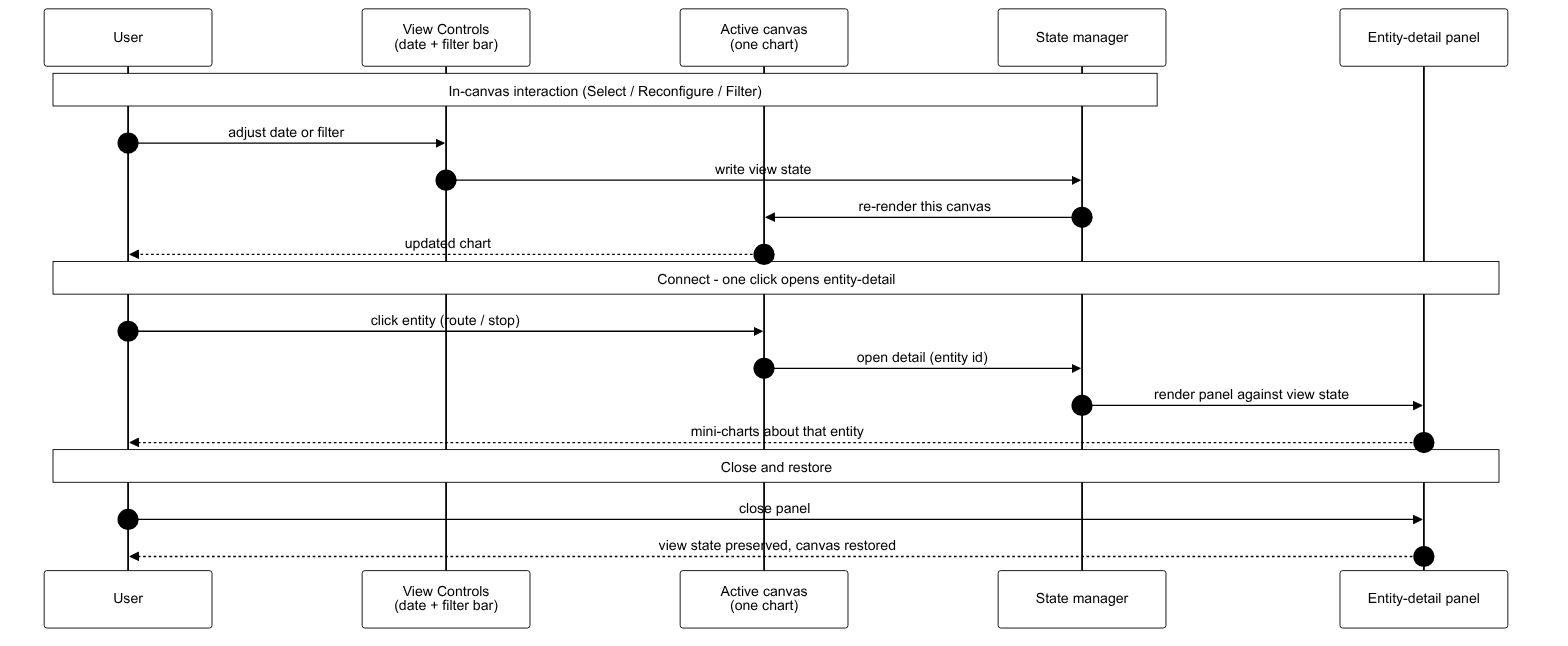
\includegraphics[width=0.92\linewidth]{images/diagrams/interaction_sequence.png}
\caption{The three interaction patterns in sequence: click-to-panel coordination, theme-scoped state persistence, and cross-theme drill-down.}
\label{fig:interaction:mcv}
\end{figure}

\subsection{Invariants}
\label{sec:solution:interaction:storytelling}

Visual storytelling is the second composed pattern. The proposed
system adopts the three storytelling devices cataloged in
Section~\ref{sec:foundations:storytelling} (three-act spine, action
title with supporting subtitle, three-to-eight-second readability
gate) as enforceable invariants on every chart in the catalog, and
adds a fourth: a zero-baseline rule for any chart whose visual
encoding is bar length. The zero-baseline rule follows from the same de-clutter
principle and rules out a known misreading mechanism in published bar
charts \cite{knaflic2015}; line charts are exempt because their
encoding is relative position, not length.

A worked example illustrates the action title in operation. A chart
titled \emph{``Route 152 carries four times the median morning-peak
ridership''} with the subtitle \emph{``Boardings per hour, top thirty
routes, weekdays January to March 2026''} reads to its finding within
seconds; the title carries the conclusion, the subtitle carries the
variables. The default palette is muted; saturated color marks the
single element the title points at; on-chart annotations (a label, a
circle, a reference line) underline the same finding inline.

The four invariants are a uniform contract across the catalog. A
single shared chart-style helper applies the muted-gray-with-single-
accent palette, suppresses unnecessary grid lines and chart borders,
enforces the title-and-subtitle hierarchy, and enforces the zero
baseline on bar-encoded charts at chart-construction time rather than
at rendering time.

\noindent\textbf{One primitive per theme.} A sixth invariant constrains the catalog at the theme level rather
than at the per-chart level: within any single analytical theme, no two
chart canvases use the same visual primitive from the Chart Selection
Rubric (Section~\ref{sec:foundations:primitives:rubric}). If the same primitive is required
for two different data subsets within a theme, the second instance
becomes a \emph{filter} on the first canvas (or a \emph{mode toggle},
or a \emph{paired-comparison overlay}), rather than a separate canvas
slot. The word \textit{invariant} is used here in the engineering
sense of a property the design will not violate, not in the sense of a
perceptual law; The constraint is a \textit{design choice} adopted for the
present project on the rationale that follows, and it is not implied
that an empirical study has shown one-primitive-per-theme to be
intrinsically more readable than its alternatives. The rationale is
informational: different chart primitives encode the analytical
quantity through different visual channels (position for scatter,
length for bar, area for treemap, hue for heatmap). A theme that
re-uses the same primitive on different data subsets adds rows that
all surface the same visual channel of difference, which is wasted
analytical surface. Forcing the second canvas to a different primitive
recruits a second visual channel and therefore a second analytical
reading of the same theme.

Three practical implications follow. First, when an exploratory pass
surfaces two candidate canvases that share a primitive, the designer
either merges them under a filter or replaces one of them with a
different primitive from the rubric. Second, the constraint forces the
designer to use the full breadth of the rubric: a theme that comprises
only ranked bars and stacked timelines is not analytically rich enough
to occupy its theme slot. Third, the constraint is theme-scoped, not
catalog-scoped: the same primitive is freely reused across themes
(four ranked bars across four themes form consistent visual
vocabulary~\cite{liu2022}; two ranked bars within one theme is
duplication).

As a concrete worked example, the route-by-hour heatmap of the Demand
and Crowding theme carries an action title above the chart, "Thirty
routes carry eighty percent of morning crowding and all peak at the
same hour", and a supporting subtitle below it, "Boardings per hour,
top thirty routes by volume, weekdays January to March 2026". The body
of the heatmap uses a muted blue-to-gray palette for the bulk of cells;
the cells in the morning-peak column of the thirty highest-volume
routes are rendered in a saturated orange that matches the action
title. A short text annotation arrow points from the title to the
orange block. The reader sees both the finding and its location in the
chart simultaneously, without having to scan the matrix unaided.

\subsection{Detail Panel}
\label{sec:solution:interaction:detail}

The entity-detail panel is the load-bearing object of the coordination
model of Section~\ref{sec:solution:interaction:mcv}. Its design
parameters fix the system's interaction grammar more than any
individual chart does, because every chart in the catalog defers to
the panel on the question \textit{``what happens when the user clicks''}.
The panel surfaces in two complementary forms. The default form is a
side panel that slides in from the right and occupies approximately
40\% of the viewport; this form is used when the entity's detail
warrants several small charts (a route, a school, an operating
company). A lighter floating-popover form, anchored to the clicked
mark, is used when the detail fits in a single KPI block plus one
sparkline (a calendar day, a time-of-day cell). The two forms share
the same content contract, the same close affordances, and the same
deep-link footer, so the analyst's mental model of \textit{``click
opens detail''} is invariant across them.

The panel body contains at most four mini-views: a one-line entity
header, a key-performance-indicator strip, a primary diagnostic mini-chart
(typically a 90-day timeline or a top-$k$ ranked bar), and optionally
one drill view (a small heatmap or a small map inset). The four-view
ceiling is a deliberate constraint: a panel that grows beyond four
views stops being a panel and starts being a second dashboard, which
defeats the panel's purpose as a quick-read surface. Entities whose
detail genuinely requires more depth route the user to a dedicated
theme via the panel's footer deep-link rather than expanding the panel
in place; the Route Detail theme of Section~\ref{sec:solution:viz:routes}
is the worked example of this routing.

Every panel carries a uniform header and a uniform footer. The header
shows the entity name, the entity type, the entity's verified-or-stubbed
provenance flag where applicable (the school dimension uses this flag
because only the eight largest universities are hand-verified per
Section~\ref{sec:solution:themes:six}), and a single close button. The
footer carries two affordances: an export-as-PDF button that captures
the panel content and a copy-shareable-link button that serializes the
active state into the browser URL so the panel content can be
reproduced from a hyperlink (this satisfies functional requirement
R10).

Two universal close affordances are honored: clicking the close button
in the header dismisses the panel, and clicking on empty space outside
the panel also dismisses it. Re-clicking on a different entity while
the panel is open replaces the panel content with the new entity
rather than stacking a second panel; the system supports at most one
panel at a time, on the rationale that side-by-side entity comparison
is a different analytical task (handled by an explicit compare-drawer
affordance, not by stacking panels).

As a concrete worked example, consider a user looking at the
Spatial-and-Connectivity theme who clicks on the Bến Thành stop on the
network-overview multi-layer hex map (chart 3.1). The side panel
slides in from the right of the screen and occupies approximately
40\% of the viewport. The panel header displays the stop name, the
stop identifier, the geographic coordinates, and the list of routes
that pass through the stop. The body contains three small charts
arranged vertically: the hourly boarding profile at the stop across
the 90-day window, a small ranked bar listing the top five routes by
boardings at the stop, and a small heatmap of day-of-week against
hour-of-day for the stop. The panel footer carries the export and
shareable-link affordances. The user has obtained a complete entity
profile in a single click and can close the panel to return to the
map without losing the rest of the theme state.

\subsection{Interaction Layers}
\label{sec:solution:interaction:composition}

The three patterns compose into a single interaction layer with a
small number of contracts. The coordination model
(Section~\ref{sec:solution:interaction:mcv}) fixes the click contract:
every click on a clickable entity in any chart opens the
entity-detail panel for the clicked entity. The visual-storytelling
invariants (Section~\ref{sec:solution:interaction:storytelling}) fix
the chart-construction contract: every chart in the catalog carries
an action title, a supporting subtitle, a muted default palette with a
single saturated accent on the focal element, and a zero baseline on
any bar-encoded chart. The entity-detail panel
(Section~\ref{sec:solution:interaction:detail}) fixes the response
contract: a panel of at most four mini-views with a uniform header
and footer, surfaced as a side panel or as a floating popover
depending on the entity's required depth.

Theme-scoped state ties the three contracts together. The user's date
range, fare-class filter, entity-multi-select, and most recent
selection are all written to a single per-theme state dictionary; the
dictionary survives navigation between charts within the theme, so the
next chart the user opens always renders against the user's active
context on its first paint. Cross-theme navigation occurs only through
the panel's footer deep-link, which migrates the relevant state slice
to the destination theme. This compositional structure realizes the
Yi (2007) Connect category through the panel and through state
persistence, rather than through simultaneous cross-chart propagation;
the result is a coherent surface in which the user can move from a
network-wide question to a single-entity answer without leaving the
theme and without losing the context that brought them there. The
interaction layer is what makes the catalog of
Section~\ref{sec:solution:viz} an analytical platform rather than a
collection of independent charts.

Four interaction patterns were considered and rejected in favor of the composition above; the cases are cataloged in Appendix~E, Section~E.2.

\subsection{Rationale}
\label{sec:solution:summary}

The proposed system responds to the requirements of Section~\ref{sec:solution:problem} through the following composition of decisions.

\begin{enumerate}
\item The Medallion warehouse architecture (Section~\ref{sec:arch:medallion}) keeps the analytical query path within the latency budget (N1) and ensures consistent identifier reconciliation across all themes (N3, N4).
\item The six analytical themes (Section~\ref{sec:solution:themes}) cover the functional capabilities R1 through R10 by partitioning the analytical surface along user-question boundaries rather than user-role boundaries.
\item The visualization catalog (Section~\ref{sec:solution:viz}) selects established primitives whose suitability is grounded in the literature surveyed in Chapter~\ref{chapter:foundations}.
\item The interaction model (click-to-entity-detail panel as the Yi (2007) Connect realization, visual storytelling as per-chart invariants, theme-scoped state for navigation continuity) bounds the user's cognitive load by routing every entity click to a single panel and reserving cross-theme navigation for the panel's explicit deep-link footer.
\item The validity boundaries of Section~\ref{sec:solution:validity} are encoded in the catalog, so no chart makes a claim the underlying data cannot support.
\end{enumerate}

The composition is the principal contribution of Phase One. Chapter~\ref{chapter:implementation} documents the parts of the proposed system that are already implemented; Chapter~\ref{chapter:conclusion} sketches the implementation plan for the remainder.
